% main.tex — versión compacta (objetivo: 12 páginas, Springer LNCS)
% Versión extendida con tablas completas: main_extended.tex
\documentclass[runningheads]{llncs}

\usepackage[T1]{fontenc}
\usepackage{graphicx}
\usepackage{subcaption}
\usepackage{amsmath}
\usepackage{booktabs}
\usepackage{multirow}
\usepackage{url}
\usepackage[section]{placeins}
\usepackage{float}

\graphicspath{{../../assets/paper/}}

\begin{document}

%% ----------------------------------------------------------------
%%  TITLE & AUTHORS
%% ----------------------------------------------------------------
\title{La segmentaci\'on de instancias, no la sem\'antica, es el factor limitante en la detecci\'on de \'arboles individuales en nubes de puntos ULS densas}

\author{Arturo~Cant\'u~Olivares\inst{1}\orcidID{0009-0007-2531-2691} \and
Diego~Sebastian~Cruz~Cervantes\inst{1}\orcidID{0009-0003-4156-972X} \and
Luis~Fernando~Maldonado\inst{1}\orcidID{0009-0005-3100-0307} \and
Jes\'us~Gabriel~Gudi\~no~Lara\inst{1}\orcidID{0009-0008-9093-9420} \and
Daniel Cantón Enriquez\inst{1}\orcidID{0000-0002-6543-5078}}

\authorrunning{A.~Cant\'u~Olivares et al.}
\titlerunning{Segmentaci\'on de instancias limita la detecci\'on de \'arboles en ULS denso}

\institute{Universidad Aut\'onoma de Quer\'etaro (UAQ), Quer\'etaro, M\'exico\\
\email{dcruz54@alumnos.uaq.mx}}

\maketitle

%% ----------------------------------------------------------------
%%  ABSTRACT
%% ----------------------------------------------------------------
\begin{abstract}
La segmentaci\'on autom\'atica de \'arboles individuales (ITS) en nubes de puntos de alta densidad obtenidas mediante escaneo l\'aser UAV (ULS) es cr\'\i{}tica para inventarios forestales escalables; sin embargo, la contribuci\'on relativa del preprocesado sem\'antico y de la segmentaci\'on de instancias al error extremo a extremo del ITS rara vez se a\'\i{}sla experimentalmente. Presentamos una comparaci\'on factorial controlada (dise\~no $3 \times 2$) entre tres estrategias de preprocesado ---sin preprocesado, Random Forest (RF) sobre features geom\'etricas y PointNet++ MSG--- combinadas con dos variantes de un segmentador volum\'etrico Watershed~3D interpretable (seeding cl\'asico por CHM y un nuevo seeding por densidad), calibrado independientemente por flujo y evaluado sobre el benchmark FOR-instance~V1 en cinco tipos de bosque. A pesar de una calidad sem\'antica casi perfecta (tree~IoU~$>$~0.97 para ambos clasificadores), el F1 de instancia alcanza un m\'aximo de 0.209, revelando una fuerte disociaci\'on entre la calidad sem\'antica y el rendimiento a nivel de instancia, donde la principal fuente de error proviene de la separaci\'on de instancias y no del preprocesado sem\'antico. Dentro de las configuraciones evaluadas, RF con features geom\'etricas supera a PointNet++ MSG en todas las combinaciones sin requerir GPU, y el seeding por densidad mejora consistentemente al CHM (+47\% en RF, +74\% en PointNet++), especialmente en canopias densas de altura uniforme donde el CHM es casi plano. Estos hallazgos son espec\'\i{}ficos de condiciones ULS densas, donde la densidad extrema de puntos y la continuidad del dosel amplifican la complejidad geom\'etrica de la separaci\'on de \'arboles individuales.

\keywords{Segmentaci\'on de \'arboles individuales \and Escaneo l\'aser UAV (ULS) \and Segmentaci\'on sem\'antica \and Watershed 3D \and Seeding por densidad \and Random Forest \and PointNet++ \and FOR-instance}
\end{abstract}
\newpage

%% ================================================================
%%  1. INTRODUCCI\'ON
%% ================================================================
\section{Introducci\'on}\label{sec:intro}

\subsection{Motivaci\'on}

Los inventarios forestales automatizados a nivel de \'arbol individual son esenciales para la estimaci\'on de carbono almacenado, el monitoreo de la biodiversidad y la silvicultura de precisi\'on. El escaneo l\'aser UAV (ULS) proporciona densidades de puntos entre uno y dos \'ordenes de magnitud superiores a las del ALS convencional ($\sim$7{,}000~pts/m$^2$ vs.\ $\sim$5~pts/m$^2$), lo que permite caracterizar \'arboles individuales, incluidas sus copas, troncos, ramas y sotobosque. Sin embargo, la segmentaci\'on autom\'atica de \'arboles individuales (ITS) en datos ULS sigue siendo un problema abierto debido al ruido en los modelos de altura, la ambig\"uedad entre copa y sotobosque, y la variabilidad estructural entre tipos de bosque, particularmente en bosques densos donde la alta densidad de puntos y la continuidad vertical hacen que múltiples árboles compartan regiones espaciales continuas.



Los pipelines de ITS suelen operar en dos etapas encadenadas: un clasificador sem\'antico que a\'\i{}sla los puntos de \'arbol respecto al suelo, sotobosque y ruido, seguido de un segmentador de instancias que asigna a cada punto de \'arbol un identificador \'unico. Los m\'etodos de aprendizaje profundo, como PointNet++~\cite{qi2017}, han generado altas expectativas respecto a la calidad sem\'antica; sin embargo, su ventaja pr\'actica frente a clasificadores cl\'asicos como Random Forest en el contexto espec\'\i{}fico del preprocesado para ITS a\'un no est\'a clara. Al mismo tiempo, los m\'etodos volum\'etricos de Watershed~3D han evolucionado m\'as all\'a del enfoque cl\'asico 2D basado en CHM~\cite{dalponte2016}, permitiendo explotar directamente la densidad vertical de puntos. A pesar de estos avances, el impacto relativo de cada etapa sobre el rendimiento extremo a extremo rara vez se ha aislado experimentalmente~\cite{qi2017,breiman2001,puliti2023}, la mayoría de los trabajos recientes en ITS se enfocan principalmente en incrementar el desempeño global mediante arquitecturas end-to-end cada vez más complejas. Sin embargo, al acoplar estrechamente la clasificación semántica y la segmentación de instancias dentro de modelos tipo black-box, resulta difícil identificar cuál de las etapas domina realmente el error final del pipeline.

Esto motiva una pregunta fundamental: en ambientes forestales ULS densos, ¿el principal límite del ITS moderno proviene de la clasificación semántica o de la separación de instancias?

\subsection{Contribuciones}

Las contribuciones de este trabajo son:

(1) un diseño factorial controlado $3 \times 2$ capaz de aislar experimentalmente la contribución relativa del preprocesado semántico y de la segmentación de instancias dentro de pipelines ITS para ambientes ULS densos;

(2) evidencia experimental de una fuerte disociación entre calidad semántica e instancia, donde valores tree IoU superiores a 0.97 no se traducen en mejoras proporcionales de segmentación individual;

(3) un análisis comparativo entre Random Forest y PointNet++ MSG bajo estrategias CHM y Density dentro de un mismo segmentador Watershed 3D interpretable; y

(4) evidencia de que el principal cuello de botella del pipeline ITS evaluado emerge de la separación de instancias y no del preprocesado semántico.


%% ================================================================
%%  2. TRABAJO RELACIONADO
%% ================================================================
\section{Trabajo Relacionado}\label{sec:related}

\subsection{Detección de árboles individuales y segmentación de instancias}

En ALS convencional (${<}10$~pts/m$^2$), el enfoque dominante para ITS detecta m\'aximos locales en el CHM y delimita copas mediante watershed~2D~\cite{popescu2002,silva2016,dalponte2016}. Estos m\'etodos se degradan en canopias densas y estratificadas, donde las copas se superponen. Los datos ULS (${\sim}10^3$--$10^4$~pts/m$^2$) habilitan enfoques volum\'etricos~3D que separan troncos adyacentes y sotobosque mediante llenado volum\'etrico, en lugar de depender de una proyecci\'on horizontal~\cite{dalponte2016}; sin embargo, pocos trabajos a\'\i{}slan la contribuci\'on del preprocesado sem\'antico respecto del segmentador de instancias. Esta brecha motiva nuestro dise\~no factorial controlado.

\subsection{Segmentación semántica de nubes de puntos forestales}

Los m\'etodos cl\'asicos emplean caracter\'\i{}sticas geom\'etricas dise\~nadas manualmente junto con Random Forest~\cite{breiman2001} o SVM~\cite{weinmann2015,weinmann2017}, mientras que los m\'etodos de aprendizaje profundo (PointNet~\cite{qi2016}, PointNet++~\cite{qi2017}) aprenden representaciones de extremo a extremo. PointNet++ ha mostrado resultados prometedores en ULS con caracter\'\i{}sticas normalizadas por altura, pero la clasificaci\'on sem\'antica se eval\'ua predominantemente como tarea final; su papel como preprocesado para ITS sigue poco estudiado.

\subsection{Benchmarks}

FOR-instance~V1~\cite{puliti2023} re'une parcelas ULS de cinco tipos de bosque distribuidos en cuatro continentes, con anotaciones sem'anticas y de instancia a nivel de punto. FOR-instanceV2~\cite{xiang2025} ampl'ia este recurso; en este trabajo evaluamos sobre V1 para mantener la comparabilidad. NeonTreeEvaluation~\cite{weinstein2021} ofrece datos multimodales, pero est'a limitado a ecosistemas de Norteam'erica.
Métodos end-to-end recientes como TreeLearn~\cite{henrich2024}, SegmentAnyTree~\cite{wielgosz2024} y ForestFormer3D~\cite{xiang2025} integran representación semántica y agrupamiento de instancias en un mismo modelo, alcanzando mejores métricas globales pero dificultando aislar qué componente domina el error final.

%% ================================================================
%%  3. DATASET
%% ================================================================
\section{Dataset}\label{sec:dataset}

\subsection{FOR-instance}

FOR-instance~V1~\cite{puliti2023} es un benchmark ULS con anotaciones sem\'anticas e de instancias a nivel de punto. Utilizamos cinco de las seis colecciones (Tabla~\ref{tab:collections}), excluyendo NIBIO2 por sobre-representar el bosque boreal noruego, lo que sesgar\'\i{}a las m\'etricas agregadas. Las densidades var\'\i{}an entre $454$ y $10\,156$~pts/m$^2$ (mediana por colecci\'on: RMIT~$473$, TUWIEN~$1\,406$, CULS~$2\,510$, SCION~$3\,064$, NIBIO~$7\,246$). La diversidad geogr\'afica y estructural es clave: NIBIO representa el 50\% del test (bosque boreal denso), mientras que RMIT y TUWIEN presentan estructuras de copa radicalmente diferentes.

\begin{table}[H]
\centering
\caption{Colecciones del dataset FOR-instance V1 utilizadas en este trabajo.}\label{tab:collections}
\begin{tabular}{llccc}
\toprule
C\'odigo & Pa\'\i{}s & Tipo de bosque & Plots test & \'Arboles GT \\
\midrule
NIBIO  & Noruega       & Boreal con\'\i{}fero (\emph{P.~abies})        & 6 & 161 \\
CULS   & Rep.\ Checa   & Templado con\'\i{}fero (\emph{P.~sylvestris}) & 1 &  20 \\
TUWIEN & Austria       & Mixto deciduo aluvial                      & 1 &  35 \\
RMIT   & Australia     & Escler\'ofilo seco (eucaliptos)             & 1 &  64 \\
SCION  & Nueva Zelanda & Plantaci\'on con\'\i{}fera (\emph{P.~radiata}) & 2 &  43 \\
\midrule
\textbf{Total} & & & \textbf{11} & \textbf{323} \\
\bottomrule
\end{tabular}
\end{table}

\subsection{Splits y reproducibilidad}\label{sec:splits}

Se utiliza el split oficial (70\% dev / 30\% test) con subdivisi\'on interna train/val (80/20\%) a nivel de plot con semilla fija, siguiendo~\cite{henrich2024,wielgosz2024}.

%% ================================================================
%%  4. METODOLOG\'IA
%% ================================================================
\section{Metodolog\'\i{}a}\label{sec:method}

\subsection{Visi\'on general del pipeline}

En lugar de proponer una nueva arquitectura ITS end-to-end, este trabajo adopta un diseño factorial interpretable que prioriza el aislamiento experimental del efecto del preprocesado semántico y la estrategia de separación de instancias sobre la maximización directa del desempeño absoluto. Watershed 3D fue seleccionado como segmentador base por su dependencia explícita de la generación geométrica de semillas, permitiendo observar cómo los errores semánticos se propagan hacia la segmentación de instancias bajo condiciones controladas.

Los flujos comparten una arquitectura de dos etapas: (1)~preprocesado sem\'antico y (2)~segmentador Watershed~3D, variadas factorialmente en cinco flujos (Fig.~\ref{fig:pipeline}). Los par\'ametros del segmentador se calibran independientemente por flujo mediante grid search sobre val (F1 de instancia, IoU~3D~$\geq 0.5$).

\begin{figure}[H]
\centering
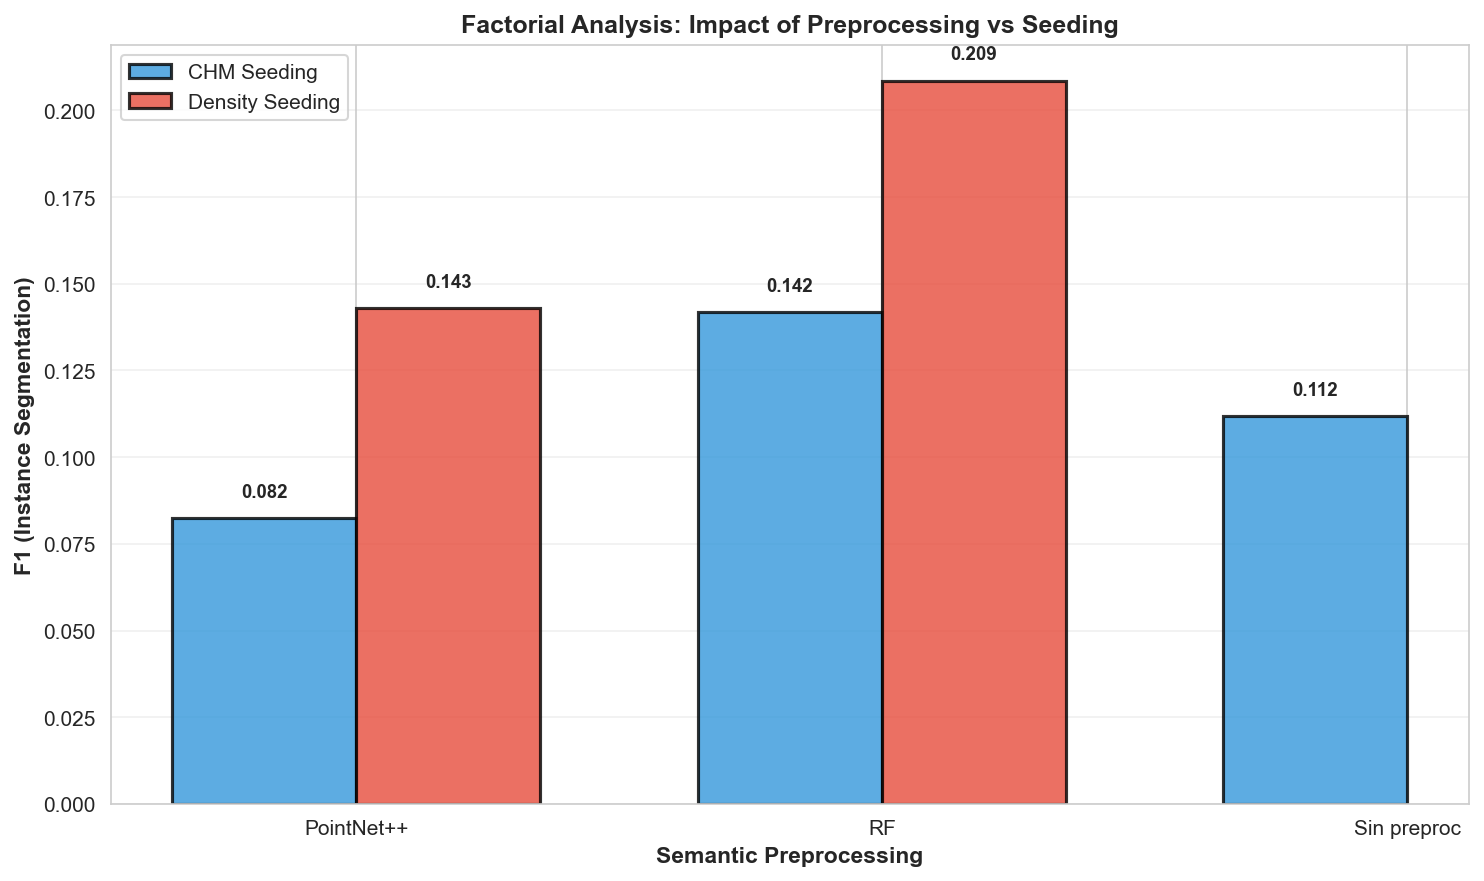
\includegraphics[width=\textwidth]{fig_05_factorial_analysis}
\caption{An\'alisis factorial: el seeding por densidad (rojo) supera al CHM (azul) en todos los m\'etodos (+47--74\%), con mejora mayor que el cambio de preprocesado (+27\%).}\label{fig:pipeline}
\end{figure}

\subsection{Flujo~A --- Sin preprocesado (baseline)}

La nube completa (excluyendo clases $\{0, 3\}$) se pasa directamente al segmentador. Todos los flujos comparten el c\'alculo de HAG a partir de un DTM interpolado sobre puntos de suelo, truncada a $[0, 50]$\,m.

\subsection{Flujo~B --- Random Forest sobre features geom\'etricas}

Cada punto se representa mediante 27 features geom\'etricas: 8 descriptores eigen-basados y 5 descriptores locales (HAG, verticalidad, rugosidad, rango vertical, intensidad normalizada), calculados a dos vecindades $k \in \{20, 50\}$, m\'as densidad volum\'etrica local ($r = 0{,}5$\,m)~\cite{weinmann2015,weinmann2017}. Se impone un radio m\'aximo de b\'usqueda de $5{,}0$\,m. El clasificador es un Random Forest ($n=200$ \'arboles, balanceo por clase) entrenado con submuestreo de $12\,000$ pts/clase/plot.

\subsection{Flujo~C --- PointNet++ MSG}

Se emplea PointNet++ MSG~\cite{qi2017} con cuatro m\'odulos Set Abstraction y cuatro Feature Propagation~\cite{yan2019pointnet2pytorch}. La entrada son 5 dimensiones por punto ($XYZ$ + HAG\_norm + intensidad), garantizando equivalencia de informaci\'on con el Flujo~B. La red se entrena durante 100 \'epocas con submuestreos de $8\,192$ puntos. En inferencia se realizan m\'ultiples pasadas con promediado de probabilidades; los puntos residuales se etiquetan por interpolaci\'on KNN ($k=3$).

\subsection{Segmentador de instancias --- Watershed 3D volum\'etrico}\label{sec:watershed}

El segmentador opera sobre los puntos clasificados como \'arbol en HAG y sigue cuatro pasos: (1)~voxelizaci\'on 3D en $(X, Y, \text{HAG})$; (2)~suavizado gaussiano 3D de la grilla de densidad; (3)~detecci\'on de semillas; y (4)~watershed volum\'etrico sobre la densidad suavizada invertida con m\'ascara de v\'oxeles ocupados~\cite{dalponte2016}. A diferencia del watershed 2D sobre CHM, el fill volum\'etrico separa correctamente troncos adyacentes y puntos de sotobosque.

\paragraph{Variante CHM (Flujos A, B, C).} Las semillas se detectan sobre la envolvente superior del volumen (equivalente a un CHM derivado del propio grid 3D) mediante \texttt{peak\_local\_max}.

\paragraph{Variante Density (Flujos D, E).} Se reemplaza el CHM por una superficie de densidad acumulada en una banda de \emph{top\_band\_m} metros bajo el v\'oxel m\'as alto de cada columna. Esta superficie refleja concentraciones locales de puntos incluso cuando el CHM es casi plano, como en bosques boreales densos de altura uniforme.

\paragraph{Calibraci\'on.}
Par\'ametros calibrados por grid search independiente por flujo (Tabla~\ref{tab:grid-search}, Fig.~\ref{fig:gridsearch}).

\begin{table}[H]
\centering
\caption{Par\'ametros \'optimos del Watershed~3D por flujo (grid search sobre val, F1 inst.\ IoU~3D~$\geq 0.5$).}\label{tab:grid-search}
\resizebox{\textwidth}{!}{%
\begin{tabular}{lcccccc}
\toprule
Par\'ametro & Espacio & A & B (RF) & C (PN++) & D (RF+Dens.) & E (PN+++Dens.) \\
\midrule
voxel\_size (m)         & $\{0.1, 0.2, 0.3\}$      & 0.2 & 0.1 & 0.1 & 0.2 & 0.3 \\
gaussian\_sigma         & $\{0.3, 0.5, 1.0\}$      & 0.3 & 0.3 & 1.0 & 0.5 & 0.3 \\
min\_crown\_radius\_m   & $\{0.5, 1.0, 1.5, 2.0\}$ & 0.5 & 1.0 & 1.5 & 2.0 & 1.5 \\
top\_band\_m            & $\{2.0, 3.0, 5.0\}$      & --- & --- & --- & 2.0 & 5.0 \\
\midrule
F1 val (medio)          &                           & 0.272 & 0.371 & 0.377 & 0.467 & 0.450 \\
\bottomrule
\end{tabular}%
}
\end{table}

\begin{figure}[H]
\centering
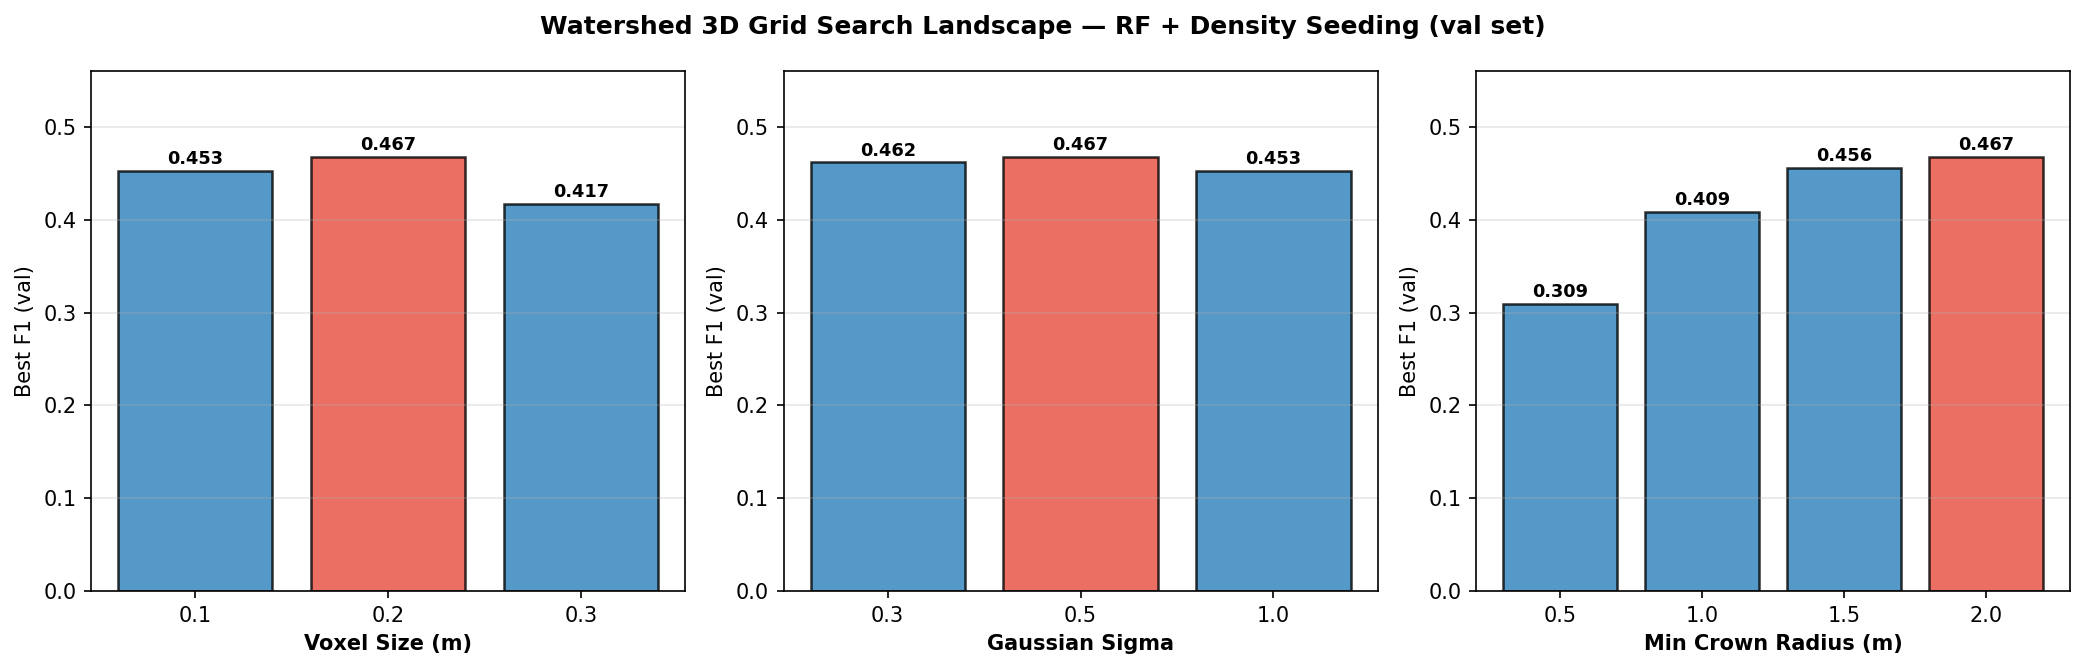
\includegraphics[width=\textwidth]{fig_v4_gridsearch_landscape}
\caption{Paisaje del grid search para el Flujo~D (RF + Density). Barras rojas: valor \'optimo. El radio m\'\i{}nimo de copa (2.0\,m) es el par\'ametro m\'as determinante.}\label{fig:gridsearch}
\end{figure}

\subsection{Detalles computacionales y reproducibilidad}
Implementación en Python (Open3D, Scikit-learn, PyTorch). RF se entrena en CPU (${\sim}16$\,min/ejecución); PointNet++ en GPU NVIDIA RTX~3060 12\,GB (${\sim}2.5$\,h, 100 épocas). Código, scripts y configuraciones: \url{https://github.com/Cantuuuu/ITS-Pipeline-Comparison}.

%% ================================================================
%%  5. PROTOCOLO DE EVALUACI\'ON
%% ================================================================
\section{Protocolo de Evaluaci\'on}\label{sec:eval}

\textbf{Sem\'antica.} Se reportan tree~IoU ($TP/(TP+FP+FN)$), seg~mIoU (promedio de IoU de ambas clases) y seg~F1 binario (\'arbol/no-\'arbol) a nivel de punto.

\textbf{Instancias.} Las instancias predichas $\{P_i\}$ se emparejan con las GT $\{G_j\}$ mediante matching \emph{greedy} por IoU~3D punto a punto con umbral $\tau = 0{,}5$, siguiendo~\cite{henrich2024,wielgosz2024}:

\begin{equation}\label{eq:iou3d}
\text{IoU}_{3D}(P_i, G_j) = \frac{|P_i \cap G_j|}{|P_i \cup G_j|}
\end{equation}

A partir del IoU~3D definido en la Ec.~\eqref{eq:iou3d}, se computan precisi\'on, recall, F1 y \emph{coverage} (fracci\'on de \'arboles GT con al menos una predicci\'on con IoU$_{3D} \geq \tau$, sin matching \'unico): la brecha Coverage~$-$~Recall indica fragmentaci\'on de copas. Reportar ambas tareas permite aislar en cu\'al etapa se concentra el error.

%% ================================================================
%%  6. RESULTADOS
%% ================================================================
\section{Resultados}\label{sec:results}

\subsection{Resultados agregados}

Las Tablas~\ref{tab:results-sem} y~\ref{tab:results-inst} presenta los resultados sobre el conjunto de test. El Flujo~D (RF + Density) alcanza el mejor desempeño agregado de segmentación de instancias (F1\,=\,0.209), mientras que el seeding por densidad mejora consistentemente ambos clasificadores respecto al CHM tradicional.

\begin{table}[H]
\centering
\caption{Calidad sem\'antica por flujo (test, nivel de punto).}\label{tab:results-sem}
\begin{tabular}{llccc}
\toprule
Flujo & Seeding & sem mIoU & tree IoU & sem F1 \\
\midrule
A --- Sin preproc.       & CHM     & --    & --    & --    \\
B --- Random Forest      & CHM     & 0.985 & 0.990 & 0.996 \\
C --- PointNet++ MSG     & CHM     & 0.974 & 0.982 & 0.994 \\
D --- Random Forest      & Density & 0.985 & 0.990 & 0.996 \\
E --- PointNet++ MSG     & Density & 0.974 & 0.982 & 0.994 \\
\bottomrule
\end{tabular}
\end{table}

\begin{table}[H]
\centering
\caption{Resultados de segmentaci\'on de instancias (test, IoU~3D~$\geq 0.5$, media $\pm$ SD sobre $n=11$~plots).}\label{tab:results-inst}
\resizebox{\textwidth}{!}{%
\begin{tabular}{llcccc}
\toprule
Flujo & Seeding & inst Prec & inst Recall & inst F1 & Coverage \\
\midrule
A --- Sin preproc.       & CHM     & $0.138 \pm 0.149$ & $0.133 \pm 0.143$ & $0.112 \pm 0.116$ & $0.133 \pm 0.143$ \\
B --- Random Forest      & CHM     & $0.394 \pm 0.402$ & $0.110 \pm 0.118$ & $0.142 \pm 0.226$ & $0.110 \pm 0.118$ \\
C --- PointNet++ MSG     & CHM     & $0.172 \pm 0.259$ & $0.060 \pm 0.079$ & $0.082 \pm 0.162$ & $0.060 \pm 0.079$ \\
D --- Random Forest      & Density & $0.418 \pm 0.291$ & $0.150 \pm 0.097$ & $\mathbf{0.209 \pm 0.161}$ & $0.150 \pm 0.097$ \\
E --- PointNet++ MSG     & Density & $0.209 \pm 0.148$ & $0.118 \pm 0.076$ & $0.143 \pm 0.109$ & $0.118 \pm 0.076$ \\
\bottomrule
\end{tabular}%
}
\vspace{1mm}
{\footnotesize $^\dagger$SD $>$ media en algunos flujos refleja distribuciones de F1 fuertemente asim\'etricas con acumulaci\'on en cero; v\'ease mediana en resultados complementarios.}
\end{table}

Ambos clasificadores logran tree~IoU~$>$~0.97, pero esta calidad no se traduce en instancia (F1 m\'aximo $0.209 \pm 0.161$), evidenciando al segmentador como cuello de botella. La alta dispersi\'on entre plots (SD comparable o superior a la media en todos los flujos) refleja la heterogeneidad estructural entre los cinco tipos de bosque evaluados. Notablemente, el density seeding reduce la variabilidad de RF (SD: $0.226 \rightarrow 0.161$), sugiriendo mayor robustez entre sitios.

\subsection{Resultados por sitio}

La Fig.~\ref{fig:semantic} muestra la clasificaci\'on sem\'antica sobre CULS~2. RF concentra errores principalmente en bordes de copa, mientras que PointNet++ produce falsos positivos aislados que posteriormente generan semillas espurias durante la segmentación.

\begin{figure}[H]
\centering
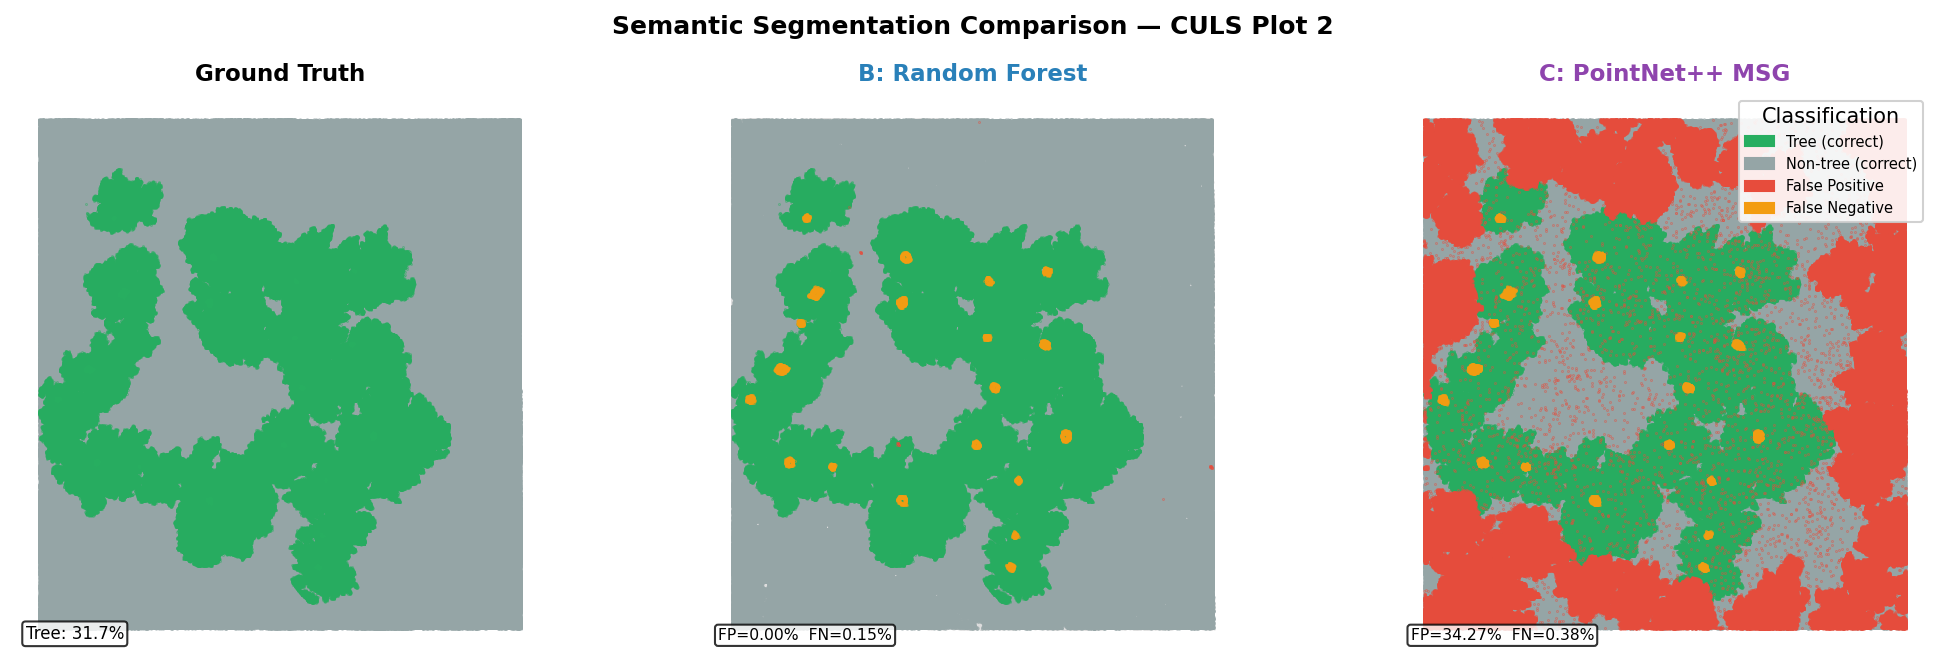
\includegraphics[width=\textwidth]{fig_v3_semantic_overlay}
\caption{Clasificaci\'on sem\'antica sobre CULS~2. Verde: \'arbol correcto; rojo: FP; naranja: FN. RF concentra errores en bordes de copa; PointNet++ produce FP aislados en suelo.}\label{fig:semantic}
\end{figure}

La Fig.~\ref{fig:f1site} muestra el F1 por sitio. CULS presenta el mejor desempeño debido a la separación clara entre copas, mientras que NIBIO representa el escenario más desafiante por su continuidad de dosel y alta densidad estructural. El seeding por densidad mejora consistentemente todos los sitios, especialmente en RMIT y TUWIEN, donde el CHM pierde capacidad discriminativa bajo estructuras de copa complejas.

\begin{figure}[H]
\centering
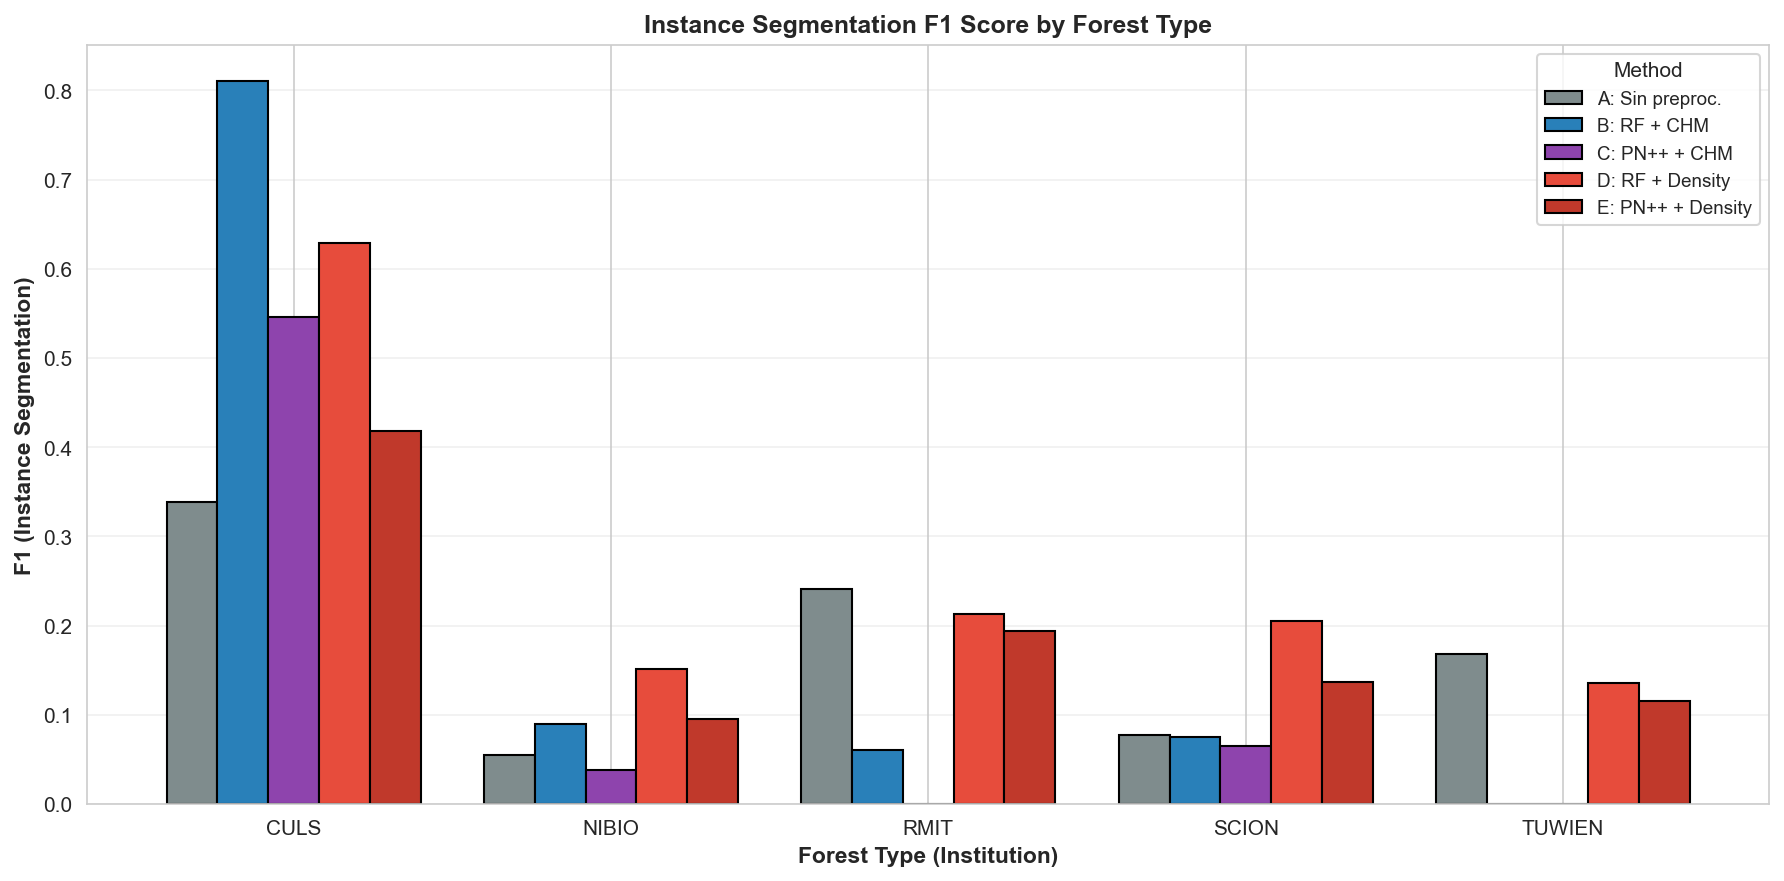
\includegraphics[width=\textwidth]{fig_02_f1_by_institution}
\caption{F1 de instancia por tipo de bosque. El Flujo~D (RF + Density, rojo) domina en todos los sitios excepto CULS (F1\,=\,0.811 con Flujo~B).}\label{fig:f1site}
\end{figure}

\subsection{Visualizaci\'on de segmentaci\'on de instancias}

Las Figs.~\ref{fig:topculs} y~\ref{fig:topnibio} muestran vistas superiores de predicciones: CULS exhibe buena separaci\'on de copas mientras que NIBIO muestra sobre-fusi\'on persistente.

\begin{figure}[H]
\centering
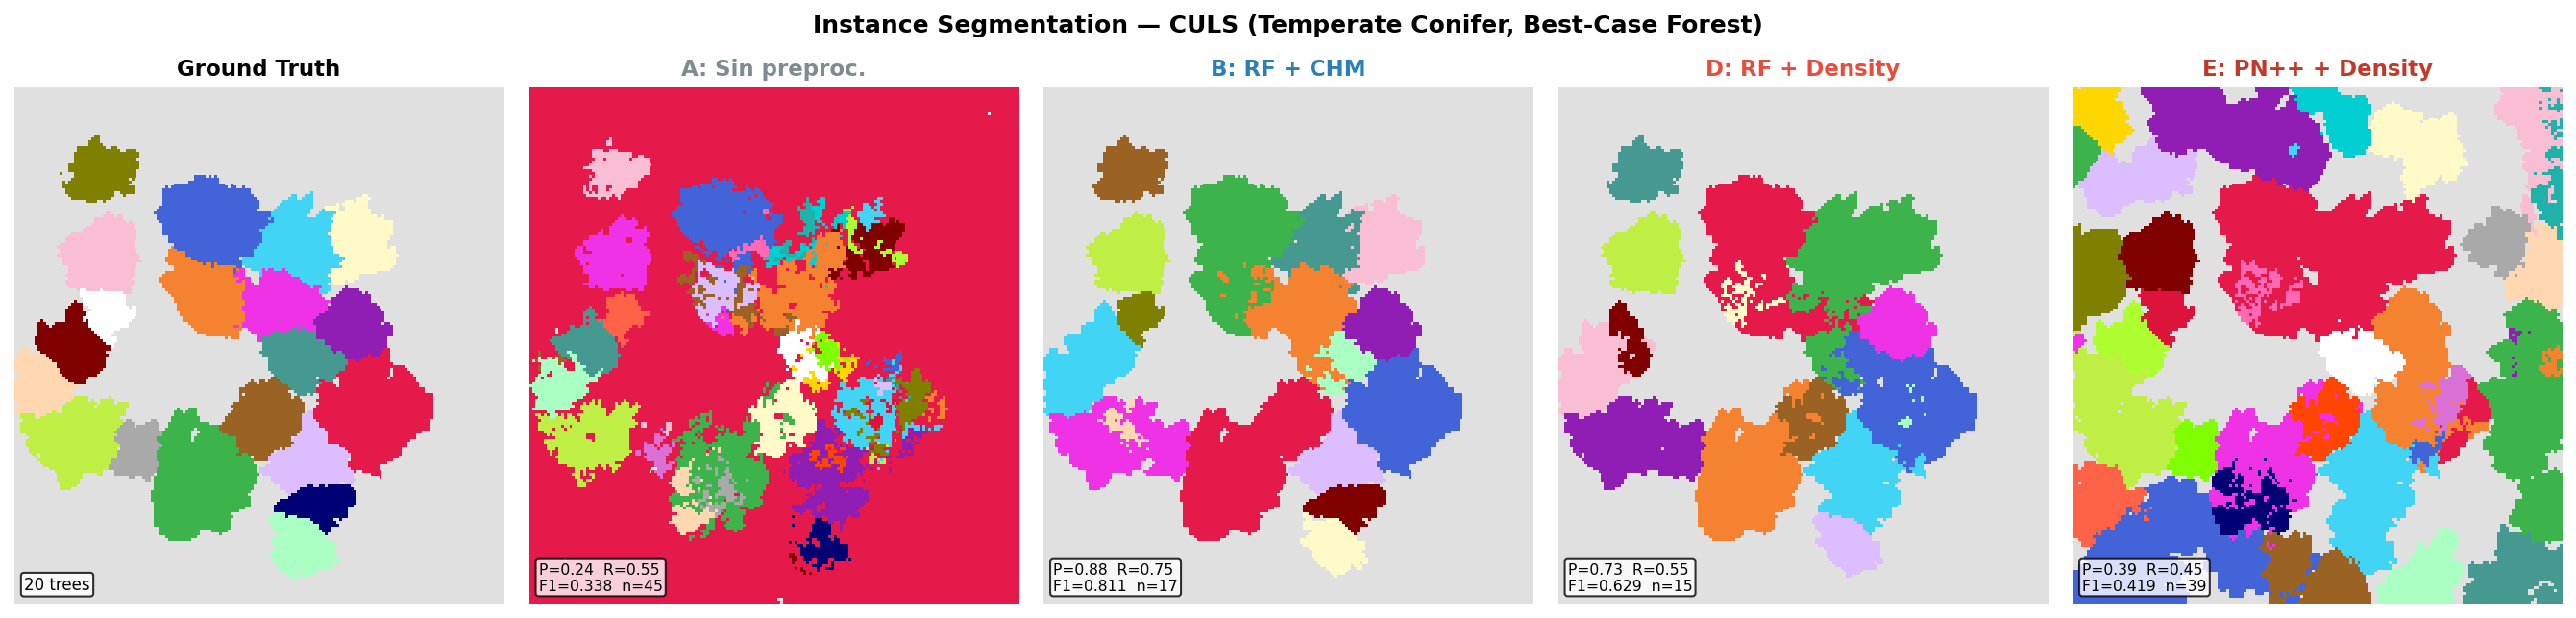
\includegraphics[width=\textwidth]{fig_v1_topview_culs}
\caption{Vista superior en CULS~2. El Flujo~D logra la mejor separaci\'on (F1\,=\,0.629); el CHM tiende a fusionar copas adyacentes.}\label{fig:topculs}
\end{figure}

\begin{figure}[H]
\centering
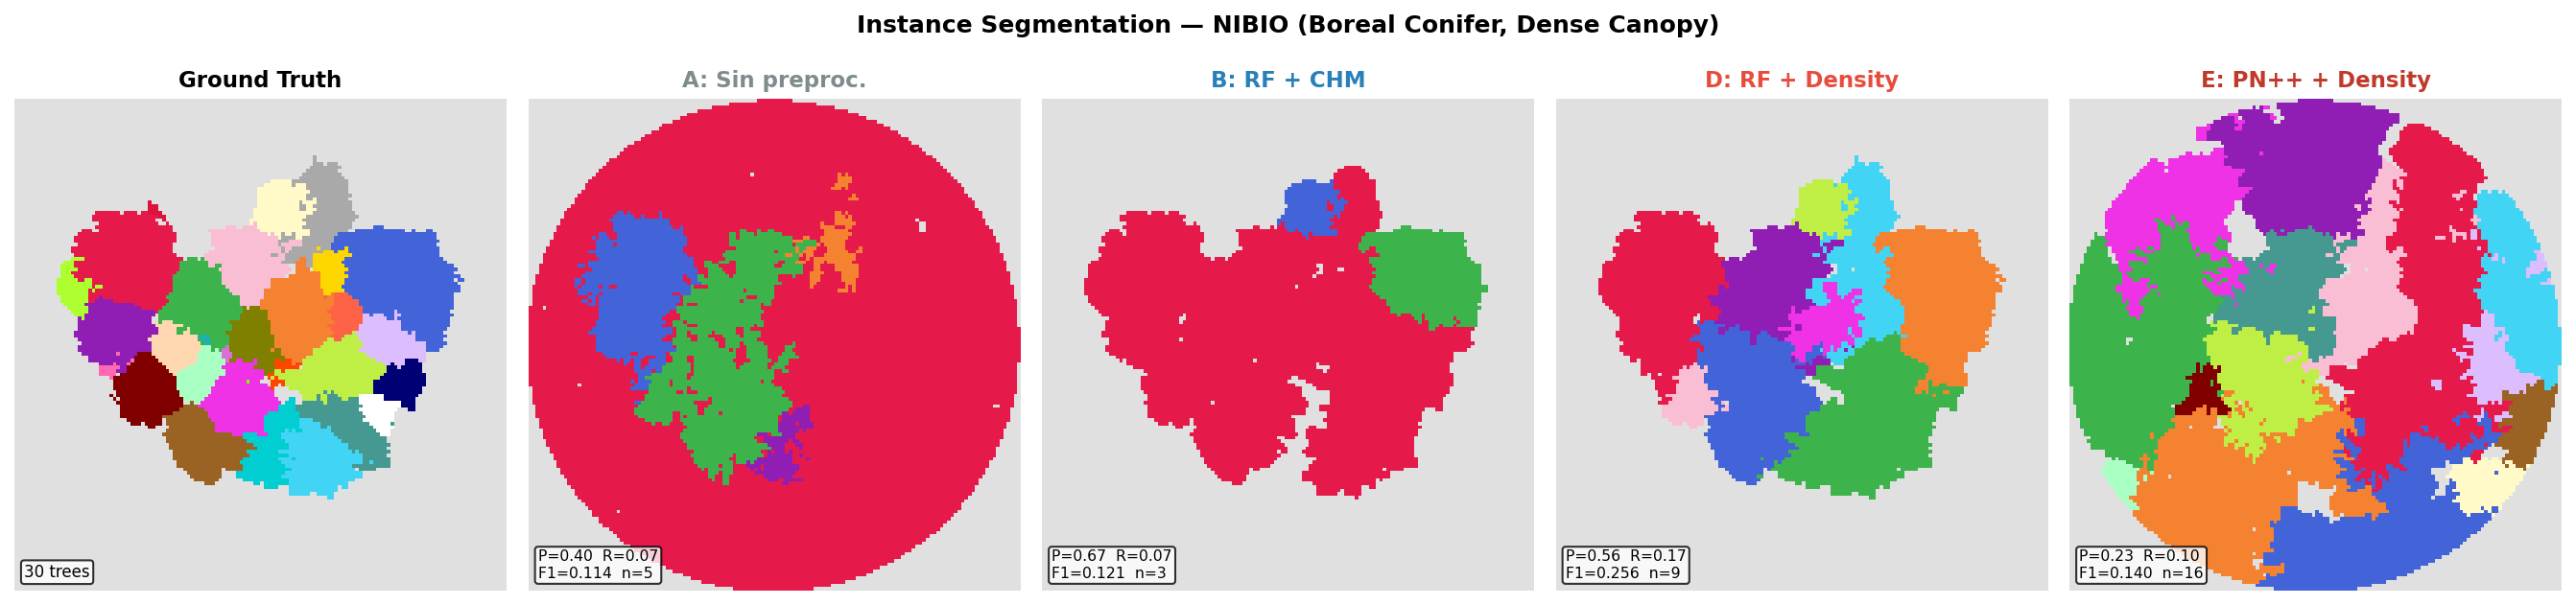
\includegraphics[width=\textwidth]{fig_v2_topview_nibio}
\caption{Vista superior en NIBIO~17 (boreal denso). Under-segmentation severo en todos los m\'etodos; F1 m\'aximo 0.256 con Flujo~D.}\label{fig:topnibio}
\end{figure}

\subsection{An\'alisis factorial: preprocesado $\times$ seeding}

\begin{table}[H]
\centering
\caption{F1 de instancia (test, media $\pm$ SD) en el dise\~no factorial. $\Delta$: mejora relativa del seeding Density sobre CHM.}\label{tab:factorial}
\begin{tabular}{lccc}
\toprule
Preprocesado & CHM & Density & $\Delta$ \\
\midrule
Sin preproc. (baseline) & $0.112 \pm 0.116$ & ---   & ---   \\
Random Forest           & $0.142 \pm 0.226$ & $\mathbf{0.209 \pm 0.161}$ & +47\% \\
PointNet++ MSG          & $0.082 \pm 0.162$ & $0.143 \pm 0.109$ & +74\% \\
\bottomrule
\end{tabular}
\end{table}

El an\'alisis factorial (Tabla~\ref{tab:factorial}, Fig.~\ref{fig:decoupling}) confirma que el cambio de seeding (CHM $\rightarrow$ Density) produce una mejora mayor (+47--74\%) que el cambio de preprocesado (baseline $\rightarrow$ RF, +27\%), identificando al segmentador como cuello de botella dominante. La interacci\'on entre ambos factores es relevante: la sem\'antica m\'as limpia de RF produce menos semillas esp\'ureas, resultando en menor sobre-segmentaci\'on (Precision RF+Density: 0.418 vs.\ PN++Density: 0.209).

\paragraph{An\'alisis de significancia estad\'\i{}stica.}
Se emplea un test de permutaci\'on exacto pareado (bilateral, $2^{11}$ permutaciones, $n=11$ plots) con intervalos bootstrap BCa al 95\% ($10\,000$ remuestreos); se prefiere sobre Wilcoxon o $t$-Student por preservar la magnitud de las diferencias y no requerir supuestos distribucionales sobre la distribuci\'on F1, fuertemente asim\'etrica con acumulaci\'on en cero. La Tabla~\ref{tab:significance} resume los resultados: RF supera a PointNet++ con significancia plena bajo CHM ($p=0.016$) y Density ($p=0.020$), y RF+Density supera al baseline ($p=0.016$). El density seeding alcanza significancia marginal ($p=0.096$ para RF, $p=0.066$ para PointNet++) limitada por $n=11$; el efecto es consistente en 8/11~plots, los IC BCa para PointNet++ excluyen el cero, y la reducci\'on de SD de F1 ($0.226 \rightarrow 0.161$ para RF) indica mayor robustez entre tipos de bosque. Validar significancia estricta del seeding requerir\'a FOR-instanceV2~\cite{xiang2025}, con mayor n\'umero de plots y diversidad.

\begin{table}[H]
\centering
\caption{Test de permutaci\'on exacto pareado (bilateral, $2^{11}$ permutaciones, $n=11$ plots) e intervalos de confianza bootstrap BCa al 95\% para diferencias en F1 de instancia.}\label{tab:significance}
\resizebox{\textwidth}{!}{%
\begin{tabular}{lcccccc}
\toprule
Comparaci\'on & $\bar{\Delta}$ F1 & SD($\Delta$) & $p_{\text{perm}}$ & IC 95\% BCa ($\Delta$) & Plots con mejora \\
\midrule
RF: CHM $\rightarrow$ Density (B vs.\ D)            & $+0.067$ & $0.119$ & $0.096^{*}$  & $[-0.004, +0.129]$ & 8/11 \\
PN++: CHM $\rightarrow$ Density (C vs.\ E)           & $+0.061$ & $0.094$ & $0.066^{*}$  & $[+0.003, +0.110]$ & 8/11 \\
Baseline $\rightarrow$ RF+Density (A vs.\ D)         & $+0.097$ & $0.103$ & $0.016^{**}$ & $[+0.027, +0.161]$ & 9/11 \\
Baseline $\rightarrow$ RF+CHM (A vs.\ B)             & $+0.030$ & $0.181$ & $0.665$      & ---                 & 7/11 \\
RF vs.\ PN++ con CHM (B vs.\ C)                      & $-0.060$ & $0.082$ & $0.016^{**}$ & ---                 & ---  \\
RF vs.\ PN++ con Density (D vs.\ E)                  & $-0.066$ & $0.077$ & $0.020^{**}$ & ---                 & ---  \\
\bottomrule
\multicolumn{6}{l}{\footnotesize $^{**}$Significativo a $\alpha = 0.05$. $^{*}$Marginalmente significativo a $\alpha = 0.10$. IC BCa: $10\,000$ remuestreos, semilla 42.}
\end{tabular}%
}
\end{table}

%% --- FIGURA 5: Semantic vs Instance decoupling ---
\begin{figure}[H]
\centering
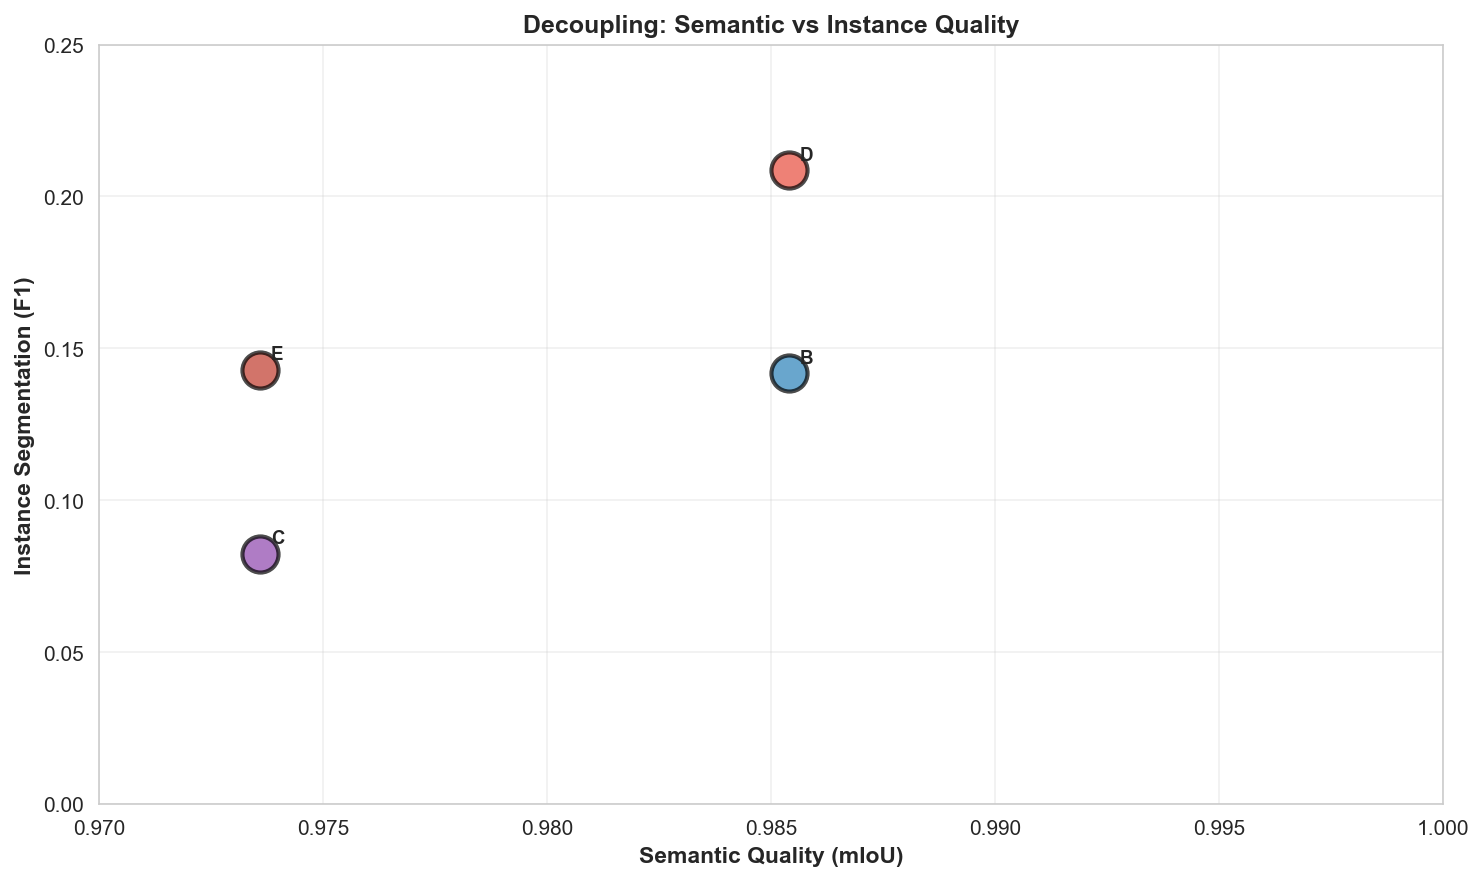
\includegraphics[width=\textwidth]{fig_03_semantic_instance_decoupling}
\caption{Desacoplamiento sem\'antico-instancia. Tree~IoU~$>$~0.97 para ambos clasificadores, pero F1 inst.\ difiere $1.7\times$ (RF vs.\ PN++ con CHM). El segmentador es el factor dominante.}\label{fig:decoupling}
\end{figure}

\subsection{Importancia de features --- Random Forest}

La HAG domina la clasificaci\'on RF con el 61.5\% de la importancia Gini acumulada en sus dos escalas ($k\!=\!50$: 0.325; $k\!=\!20$: 0.290), confirmando que la altura sobre el suelo es el predictor primario de la separaci\'on \'arbol/no-\'arbol. La verticalidad (0.087) y la rugosidad (0.072) a escala gruesa aportan informaci\'on geom\'etrica complementaria.

%% ================================================================
%%  7. DISCUSI\'ON
%% ================================================================
\section{Discusi\'on}\label{sec:discussion}

\subsection{El segmentador como cuello de botella}

La Fig.~\ref{fig:vprofile} ilustra c\'omo el Flujo~D asigna correctamente puntos de tronco y ramas en CULS~2, mientras que la proyecci\'on 2D del CHM confundir\'\i{}a estos puntos. El fill volum\'etrico del Watershed~3D es la diferencia estructural decisiva. Cabe notar que la calibraci\'on independiente por flujo (Tabla~\ref{tab:grid-search}) produce par\'ametros \'optimos diferentes: el density seeding prefiere v\'oxeles m\'as gruesos ($0.2$--$0.3$\,m) para acumular suficiente masa de puntos en la banda superior, mientras que el CHM requiere alta resoluci\'on ($0.1$\,m) para preservar los picos locales de la envolvente. Esta divergencia no es un sesgo experimental sino una restricci\'on geom\'etrica de cada estrategia de seeding; la calibraci\'on independiente permite que cada pipeline alcance su techo de rendimiento.

\begin{figure}[H]
\centering
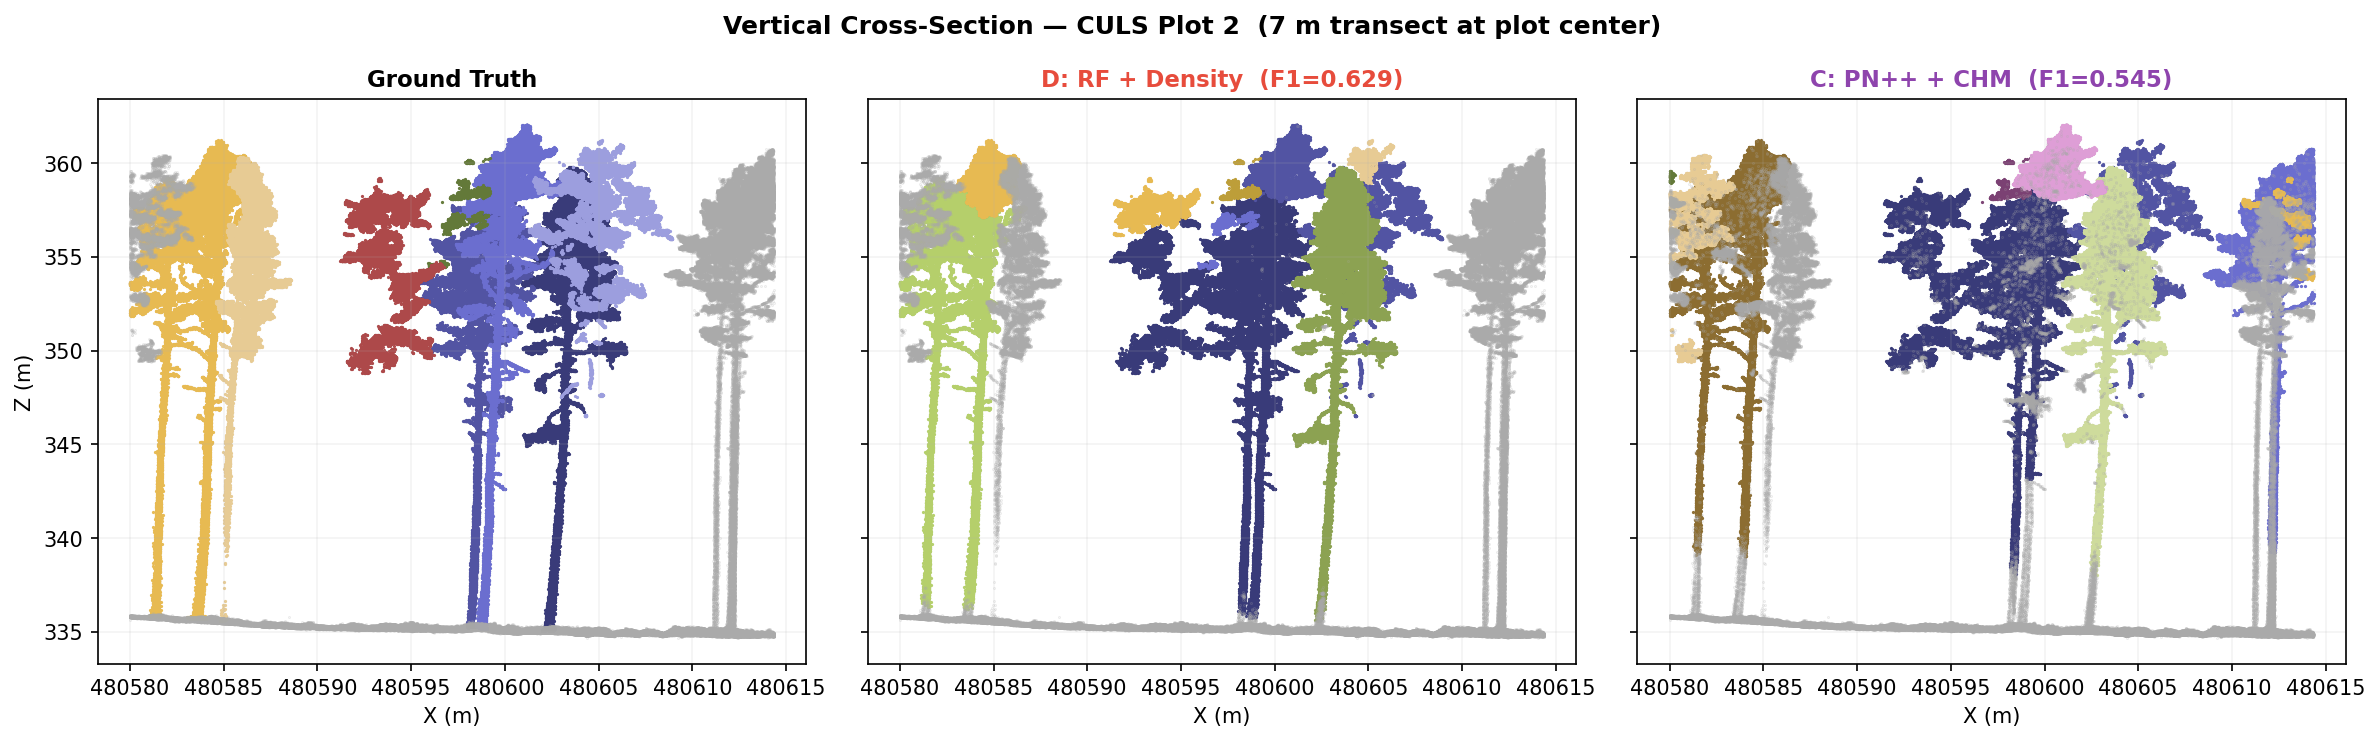
\includegraphics[width=\textwidth]{fig_v5_vertical_profile}
\caption{Perfil vertical (7\,m) en CULS~Plot~2. El Flujo~D (centro) separa correctamente los \'arboles usando fill volum\'etrico; PointNet++ + CHM (derecha) confunde troncos compartidos.}\label{fig:vprofile}
\end{figure}

El hallazgo central (Fig.~\ref{fig:decoupling}) es que la sem\'antica casi perfecta (tree~IoU~$>$~0.97) no se traduce en calidad de instancia proporcional (F1 m\'aximo 0.209). El principal factor limitante observado en el pipeline evaluado es la capacidad de separación de instancias bajo estructuras de copa altamente continuas y superpuestas. El an\'alisis factorial confirma que la inversi\'on m\'as rentable en un pipeline ITS de dos etapas no est\'a en mejorar la sem\'antica --- que RF ya supera ampliamente --- sino en mejorar el segmentador de instancias. El efecto es dependiente del sitio: en CULS (copas separadas), RF+CHM alcanza F1\,=\,0.811 y el Density seeding no aporta mejora sustancial; en NIBIO, RMIT y TUWIEN, donde las copas se superponen, el CHM falla sistem\'aticamente y el Density seeding es necesario para obtener rendimiento no trivial.

La dificultad observada refleja un problema geométrico más general en ULS denso: cuando las copas se superponen y la altura es uniforme, múltiples árboles comparten una misma masa volumétrica de puntos, reduciendo la separabilidad incluso antes de aplicar un algoritmo específico. Cualquier método basado principalmente en señales geométricas locales enfrentará dificultades similares; Watershed~3D funciona aquí como instrumento interpretable para exponer esta limitación estructural más que como una afirmación de optimalidad algorítmica. En adquisiciones ALS de menor densidad, donde las copas son más dispersas, la relación entre error semántico e instancia podría diferir.

Aunque métodos recientes como TreeLearn~\cite{henrich2024}, SegmentAnyTree~\cite{wielgosz2024} y ForestFormer3D~\cite{xiang2025} probablemente alcancen mejores métricas absolutas, el objetivo de este trabajo no es competir contra arquitecturas estado-del-arte, sino analizar la relación entre calidad semántica y separación de instancias dentro de un pipeline interpretable.

\subsection{RF vs.\ PointNet++: viabilidad sin GPU y generalizaci\'on}

RF obtiene mejores resultados que PointNet++ en las configuraciones evaluadas, particularmente bajo escenarios con alta heterogeneidad estructural entre sitios. Esta ventaja no se explica por sem\'antica superior (brecha en tree~IoU~$<$~1\,pp), sino por mejor interacci\'on con el segmentador: los errores de RF son falsos positivos de borde de copa, mientras que PointNet++ genera falsos positivos aislados en suelo que producen semillas esp\'ureas. Adem\'as, RF se entrena e infiere en CPU (${\sim}16$\,min) sin requerir GPU.

PointNet++ muestra ca\'\i{}da severa en RMIT y TUWIEN (F1\,=\,0.000 con CHM), debido a que su submuestreo global de $8\,192$ puntos no captura adecuadamente sitios con densidades y morfolog\'\i{}as muy diferentes a los datos de entrenamiento (dominados por NIBIO boreal). RF, al operar sobre features locales, generaliza mejor entre tipos de bosque diversos.

Esta ventaja se observa dentro de las configuraciones evaluadas y no debe leerse como superioridad general de clasificadores clásicos sobre deep learning (cf.\ §7.3); aún así, refuerza la hipótesis central de desacoplamiento, ya que mejoras semánticas no se traducen en mejoras proporcionales a nivel de instancia.

\subsection{Limitaciones}

\paragraph{Tama\~no y balance del conjunto de evaluaci\'on.}
El conjunto de test comprende 11~plots y 323~\'arboles GT, con una concentraci\'on significativa en un solo tipo de bosque: NIBIO (boreal con\'\i{}fero) aporta 6 de 11 plots (${\sim}50\%$) y 161 de 323 \'arboles (${\sim}50\%$), mientras que CULS, TUWIEN y RMIT contribuyen un \'unico plot cada uno. Esta distribuci\'on introduce dos efectos cuantificables: (i)~alta varianza en las estimaciones por sitio --- los intervalos de confianza bootstrap al 95\% de F1 para el mejor flujo (D) abarcan $[0.128, 0.314]$, reflejando que sitios individuales como CULS (F1\,=\,0.629) o NIBIO\_5 (F1\,=\,0.000) dominan la dispersi\'on; y (ii)~posible sesgo en las m\'etricas agregadas hacia el comportamiento en bosque boreal denso, que es el escenario m\'as desafiante para todos los m\'etodos.

\paragraph{An\'alisis de errores de segmentaci\'on.}
El presente trabajo cuantifica el rendimiento del segmentador mediante F1, precisi\'on, recall y coverage, pero no descompone sistem\'aticamente los errores en sobre-segmentaci\'on (un \'arbol GT fragmentado en m\'ultiples predicciones) e infra-segmentaci\'on (m\'ultiples \'arboles GT fusionados en una sola predicci\'on). Si bien las columnas \texttt{over\_seg} y \texttt{under\_seg} se registran en los resultados por plot, un an\'alisis formal de la naturaleza del error --- incluyendo la relaci\'on entre tama\~no de copa, densidad local y tipo de error predominante --- queda fuera del alcance de este estudio y se propone como trabajo futuro.

\paragraph{Otras limitaciones.}
PointNet++ se eval\'ua con una \'unica configuraci\'on de hiperpar\'ametros; una b\'usqueda exhaustiva podr\'\i{}a mejorar su rendimiento. Por esta raz\'on, las comparaciones entre RF y PointNet++ deben interpretarse principalmente como observaciones dentro del pipeline experimental evaluado y no como una comparaci\'on definitiva entre paradigmas cl\'asicos y deep learning para segmentaci\'on forestal. Las conclusiones sobre el cuello de botella son espec\'\i{}ficas al Watershed~3D volum\'etrico; otros segmentadores (TreeLearn~\cite{henrich2024}, SegmentAnyTree~\cite{wielgosz2024}) podr\'\i{}an mostrar una relaci\'on diferente. No obstante, los patrones de error observados --- especialmente la fusi\'on de copas adyacentes en canopias continuas --- sugieren una dificultad geom\'etrica m\'as amplia para la separaci\'on de instancias en ULS denso. Los resultados son espec\'\i{}ficos a datos ULS ($454$--$10\,156$~pts/m$^2$); las conclusiones presentadas deben interpretarse espec\'\i{}ficamente dentro del contexto de nubes ULS densas y no como una caracterizaci\'on universal del comportamiento de pipelines ITS sobre todas las modalidades LiDAR. Asimismo, este trabajo no busca establecer una comparaci\'on cuantitativa exhaustiva frente a arquitecturas estado-del-arte recientes, sino proporcionar una evaluaci\'on factorial interpretable orientada a identificar la distribuci\'on estructural del error dentro del pipeline ITS.

%% ================================================================
%%  8. CONCLUSIONES
%% ================================================================
\section{Conclusiones}\label{sec:conclusions}

Mediante un dise\~no factorial $3 \times 2$ sobre FOR-instance~V1, demostramos que: (1)~el segmentador de instancias, no el preprocesado sem\'antico, es el cuello de botella principal del pipeline ITS; (2)~Random Forest con features geom\'etricas supera significativamente a PointNet++ MSG en todas las combinaciones evaluadas ($p=0.016$, test de permutaci\'on exacto), sin requerir GPU; y (3)~el seeding por densidad de copa mejora consistentemente al seeding CHM (+47\% para RF, +74\% para PointNet++), con significancia marginal ($p=0.096$ y $p=0.066$, respectivamente) limitada por el tama\~no muestral del benchmark ($n=11$ plots), siendo especialmente efectivo en bosques densos de altura uniforme.

La combinación RF + Watershed~3D Density alcanza el mejor F1 de instancia (0.209 en test), estableciendo una línea base robusta y eficiente. La brecha entre calidad semántica y calidad de instancia sugiere que las mejoras más impactantes en ITS vendrán de segmentadores capaces de separar copas adyacentes en canopias densas mediante priors geométricos, arquitecturas end-to-end o estrategias de seeding más adaptativas.

Más que proponer un método competitivo, este trabajo aporta una disección experimental interpretable del pipeline ITS bajo ULS denso. Trabajo futuro: comparación con TreeLearn~\cite{henrich2024} y SegmentAnyTree~\cite{wielgosz2024}, extensión a FOR-instanceV2~\cite{xiang2025}, seeding adaptativo CHM/densidad según variabilidad local de altura, y análisis formal de sobre- vs.\ infra-segmentación por tipo de bosque.
%% ================================================================
%%  REFERENCIAS
%% ================================================================
\begin{thebibliography}{10}

\bibitem{puliti2023}
Puliti, S., et al.:
FOR-instance: a UAV laser scanning benchmark dataset for semantic and instance segmentation of individual trees.
arXiv preprint arXiv:2309.01279 (2023).
DOI: 10.5281/zenodo.8287792

\bibitem{qi2017}
Qi, C.R., Yi, L., Su, H., Guibas, L.J.:
PointNet++: Deep hierarchical feature learning on point sets in a metric space.
In: Advances in Neural Information Processing Systems (NeurIPS), pp.~5099--5108 (2017)

\bibitem{qi2016}
Qi, C.R., Su, H., Mo, K., Guibas, L.J.:
PointNet: Deep learning on point sets for 3D classification and segmentation.
In: IEEE Conference on Computer Vision and Pattern Recognition (CVPR), pp.~652--660 (2017)

\bibitem{yan2019pointnet2pytorch}
Yan, X.:
\texttt{Pointnet\_Pointnet2\_pytorch}: PyTorch implementation of PointNet and PointNet++.
GitHub repository, \url{https://github.com/yanx27/Pointnet_Pointnet2_pytorch} (2019). Accedido 2026-04

\bibitem{breiman2001}
Breiman, L.:
Random Forests.
Machine Learning \textbf{45}(1), 5--32 (2001)

\bibitem{weinstein2021}
Weinstein, B.G., Marconi, S., Bohlman, S., Zare, A., White, E.:
A benchmark dataset for canopy crown detection and delineation in co-registered airborne RGB, LiDAR and hyperspectral imagery from the National Ecological Observation Network.
PLOS Computational Biology \textbf{17}(7), e1009180 (2021).
DOI: 10.1371/journal.pcbi.1009180

\bibitem{silva2016}
Silva, C.A., Hudak, A.T., Vierling, L.A., et al.:
Imputation of individual longleaf pine (\emph{Pinus palustris} Mill.) tree attributes from field and LiDAR data.
Canadian Journal of Remote Sensing \textbf{42}(5), 554--573 (2016)

\bibitem{popescu2002}
Popescu, S.C., Wynne, R.H., Nelson, R.F.:
Estimating plot-level tree heights with lidar: local filtering with a canopy-height based variable window size.
Computers and Electronics in Agriculture \textbf{37}(1--3), 71--95 (2002)

\bibitem{dalponte2016}
Dalponte, M., Coomes, D.A.:
Tree-centric mapping of forest carbon density from airborne laser scanning and hyperspectral data.
Methods in Ecology and Evolution \textbf{7}(10), 1236--1245 (2016)

\bibitem{xiang2025}
Xiang, B., et al.:
ForestFormer3D: A unified framework for end-to-end segmentation of forest LiDAR 3D point clouds.
In: IEEE/CVF International Conference on Computer Vision (ICCV), Honolulu, Hawaii (2025).
arXiv:2506.16991

\bibitem{weinmann2015}
Weinmann, M., Jutzi, B., Hinz, S., Mallet, C.:
Semantic point cloud interpretation based on optimal neighborhoods, relevant features and efficient classifiers.
ISPRS Journal of Photogrammetry and Remote Sensing \textbf{105}, 286--304 (2015)

\bibitem{weinmann2017}
Weinmann, M., Jutzi, B., Mallet, C., Weinmann, M.:
Geometric features and their relevance for 3D point cloud classification.
ISPRS Annals of the Photogrammetry, Remote Sensing and Spatial Information Sciences \textbf{IV-1/W1}, 157--164 (2017)


\bibitem{henrich2024}
Henrich, J., et al.:
TreeLearn: A deep learning method for segmenting individual trees from ground-based LiDAR forest point clouds.
Ecological Informatics \textbf{84}, 102888 (2024).
DOI: 10.1016/j.ecoinf.2024.102888. arXiv:2309.08471

\bibitem{wielgosz2024}
Wielgosz, M., Puliti, S., Xiang, B., Schindler, K., Astrup, R.:
SegmentAnyTree: A sensor and platform agnostic deep learning model for tree segmentation using laser scanning data.
Remote Sensing of Environment \textbf{313}, 114367 (2024).
DOI: 10.1016/j.rse.2024.114367. arXiv:2401.15739


\end{thebibliography}

\end{document}
